\chapter{Superposition, and Multipass}
\label{c:super.multi}

\index{superposition}\index{multipass}
This chapter covers two concepts: \vn{superposition} (\sref{s:super})
and \vn{multipass} (\sref{s:multipass}) \vn{Superposition} is used
when elements overlap spatially.  \vn{Multipass} is used when an
element is ``shared'' between branches such as the interaction region
shared by two storage rings, or when a beam goes through the same
physical element in a branch multiple times as in an energy recovery
linac.

In both cases, \vn{lord} and \vn{slave} elements (\sref{s:lord.slave})
are constructed by \bmad to hold the necessary information. In both
cases, the \vn{lord} elements will represent the ``physical'' element
while the \vn{slave} elements will embody the ``beam path''.

%-----------------------------------------------------------------------------
\section{Superposition}
\label{s:super}
\index{superimpose|hyperbf}

  \begin{figure}[tb]
  \centering 
  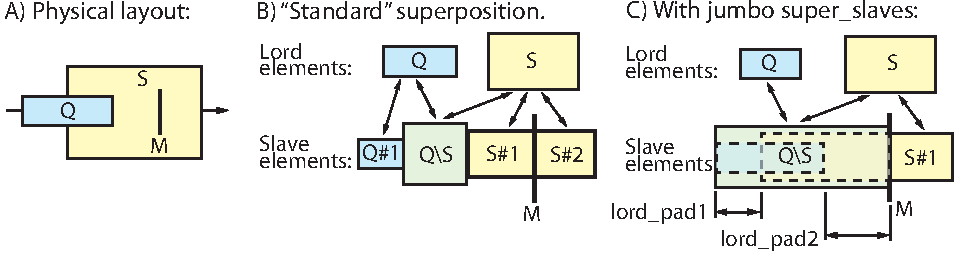
\includegraphics[width=0.95\textwidth]{superimpose-example.pdf} 
  \caption[Superposition example.]
{Superposition example. A) The physical layout involves a quadrupole
partially inside a solenoid. B) The standard superposition procedure
involves creating \vn{super_slave} elements whose edges are at the
boundaries where the physical elements overlap. C) When jumbo
\vn{super_slaves} are created, the \vn{super_slaves} span the entire
space where elements overlap.}
  \label{f:super.ex}
  \end{figure}

In practice the field at a particular point in the lattice may be due
to more than one physical element. One example of this is a quadrupole
magnet inside a larger solenoid magnet as shown in
\fig{f:super.ex}A. \bmad has a mechanism to handle this using what is
called ``superposition''. A simple example shows how this works (also
see section \sref{s:lord.slave}):
\begin{example}
  Q: quad, l = 4
  D: drift, l = 12
  S: solenoid, l = 8, superimpose, ref = Q, ele_origin = beginning
  M: marker, superimpose, ref = S, offset = 1
  lat: line = (Q, D)
  use, lat
\end{example}
The \vn{superimpose} attribute of element \vn{S} superimposes \vn{S}
over the lattice \vn{(Q, D)}. The placement of \vn{S} is such that the
beginning of \vn{S} is coincident with the center of \vn{Q} (this is
is explained in more detail below). Additionally, a marker \vn{M} is
superimposed at a distance of +1~meter from the center of \vn{S}. The
tracking part of the lattice (\sref{s:lord.slave}) looks like:
\begin{example}
        Element   Key         Length  Total     
  1)    Q{\#}1       Quadrupole   2        2
  2)    Q{\B}S       Sol_quad     2        4
  3)    S{\#}1       Solenoid     3        7
  4)    M         Marker       0      
  4)    S{\#}2       Solenoid     3       10
  5)    D{\#}2       Drift        4       14
\end{example}
What \bmad has done is to split the original elements \vn{(Q, D)} at
the edges of \vn{S} and then \vn{S} was split where \vn{M} is
inserted. The first element in the lattice, \vn{Q\#1}, is the part of
\vn{Q} that is outside of \vn{S}. Since this is only part of \vn{Q},
\bmad has put a \vn{\#1} in the name so that there will be no
confusion. (\vn{\#} has no special meaning other than the fact that
\bmad uses it for mangling names). The next element, \vn{Q{\B}S}, is
the part of \vn{Q} that is inside \vn{S}. \vn{Q{\B}S} is a combination
solenoid/quadrupole element as one would expect. \vn{S{\#}1} is the
part of \vn{S} that is outside \vn{Q} but before \vn{M}. This element
is just a solenoid. Next comes \vn{M}, \vn{S{\#}1}, and finally
\vn{D\#2} is the rest of the drift outside \vn{S}.

In the above example, \vn{Q} and \vn{S} will be \vn{super_lord}
elements (\vn{s:lord.slave}) and four elements in the tracking
part of the lattice will be \vn{super_slave} elements. This is
illustrated in \fig{f:super.ex}B.

Notice that the name chosen for the \vn{sol_quad} element \vn{Q{\B}S}
is dependent upon what is being superimposed upon what. If \vn{Q} had
been superimposed upon \vn{S} then the name would have been \vn{S{\B}Q}.

When \bmad sets the element class for elements created from
superpositions, \bmad will set the class of the element to something
other than an \vn{em_field} element (\sref{s:em.field}) if
possible. If no other possibilities exist, \bmad will use
\vn{em_field}. For example, a \vn{quadrupole} superimposed with a
\vn{solenoid} will produce a \vn{sol_quad} element but a \vn{solenoid}
superimposed with a \vn{rfcavity} element will produce an
\vn{em_field} element since there is no other class of element that
can simultaneously handle solenoid and RF fields.

  \begin{figure}[tb]
  \centering 
  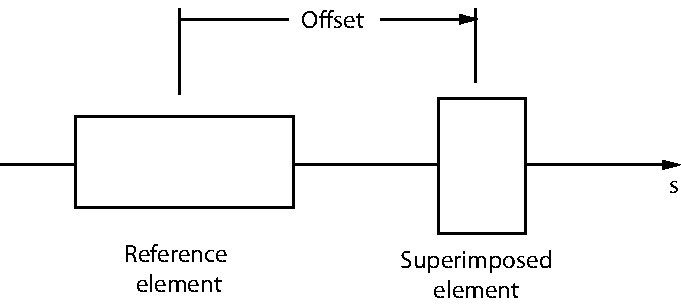
\includegraphics[width=0.8\textwidth]{superimpose.pdf} 
  \caption[Superposition Offset.]{
The superposition offset is the distance from the origin point of the
reference element to the origin point of the element being
superimposed.
  }
  \label{f:superimpose}
  \end{figure}

With the lattice broken up like this \bmad has constructed something
that can be easily analyzed. However, the original elements \vn{Q} and
\vn{S} still exist within the lord section of the lattice. \bmad has
bookkeeping routines so that if a change is made to the \vn{Q} or
\vn{S} elements then these changes can get propagated to the
corresponding slaves. It does not matter which element is
superimposed. Thus, in the above example, \vn{S} could have been put
in the Beam Line (with a drift before it) and \vn{Q} could then have
been superimposed on top and the result would have been the same
(except that the split elements could have different names).

If an element has zero length (for example, a
\vn{marker} element), is superimposed, or is superimposed upon, then the
element will remain in the tracking part of the lattice and there will be
no corresponding lord element. See \fig{f:super.ex}.
 
Superimpose syntax:
\begin{example}
  Q: quad, superimpose, ...       ! Superimpose element Q/
  Q: quad, superimpose = T, ...   ! Same as above.
  Q: quad, ...                    ! First define element Q ...
  Q[superimpose] = T              !   ... and then superimpose.
  Q[superimpose] = F              ! Turn off superposition.
\end{example}

The placement of a superimposed element is illustrated in
\fig{f:superimpose}. The placement of a superimposed element is
determined by three factors: An origin point on the superimposed
element, an origin point on the reference element, and an offset between
the points. The attributes that determine these three quantities are:
\index{ref}\index{offset}
\index{ref_origin}\index{ele_origin}
\begin{example}
  create_jumbo_slave = <Logical>     ! See \sref{s:jumbo.slave}
  ref          = <lattice_element>
  offset       = <length>            ! default = 0
  ele_origin   = <origin_location>   ! Origin pt on element.
  ref_origin   = <origin_location>   ! Origin pt on ref element.
\end{example}
\vn{ref} sets the reference element. If \vn{ref} is not present then
the start of the lattice is used (more precisely, the start of branch
0 (\sref{s:branch.def})). The location of the origin points are
determined by the setting of \vn{ele_origin} and \vn{ref_origin}.  The
possible settings for these parameters are
\begin{example}
  beginning       ! Beginning (upstream) edge of element
  center          ! Center of element. Default.
  end             ! End (downstream) edge of element
\end{example}
\vn{center} is the default setting.
\vn{offset} is the longitudinal offset
between the origin points. The default offset is zero.

Note: There is an old syntax, deprecated but still supported for now,
where the origin points were specified by the appearance of:
\begin{example}
  ele_beginning         ! Old syntax. Do not use.
  ele_center            ! Old syntax. Do not use.
  ele_end               ! Old syntax. Do not use.
  ref_beginning         ! Old syntax. Do not use.
  ref_center            ! Old syntax. Do not use.
  ref_end               ! Old syntax. Do not use.
\end{example}
For example, ``ele_origin = beginning'' in the old syntax would be ``ele_beginning''.

\index{drift}
\index{overlay}\index{group}\index{girder}
The element begin superimposed may be any type of element except
\vn{drift}, \vn{group}, \vn{overlay}, and \vn{girder} control
elements. The reference element used to position a superimposed element
may be a \vn{group} or \vn{overlay} element as long as the \vn{group} or
\vn{overlay} controls the attributes of exactly one element. In this case,
the controlled element is used as the reference element.

\index{geometry}\index{open}
A superimposed element that extends beyond either end of the lattice
will be wrapped around so part of the element will be at the beginning
of the lattice and part of the element will be at the end. For
consistency's sake, this is done even if the \vn{geometry} is set to
\vn{open} (for example, it is sometimes convenient to treat a circular
lattice as linear). Example:
\begin{example}
  d: drift, l = 10
  q: quad, l = 2, superimpose
  machine: line = (d)
  use, machine
\end{example}
The lattice will have three elements in the tracking section:
\begin{example}
        Element   Key           Length
  3)    Q{\#}2       Quadrupole    1
  2)    D{\#}1       Drift         8
  1)    Q{\#}1       Quadrupole    1
\end{example}
The lord section of the lattice will have the element \vn{Q}. 

To superimpose a zero length element ``\vn{S}'' next to a zero length
element ``\vn{Z}'', and to make sure that \vn{S} will be on the
correct side of \vn{Z}, set the \vn{ref_origin} appropriately.
For example:
\begin{example}
  S1: marker, superimpose, ref = Z, ref_origin = beginning
  S2: marker, superimpose, ref = Z, ref_origin = end
  Z: marker
\end{example}
This will place \vn{S1} upstream and \vn{S2} downstream of \vn{Z}.  If
\vn{ref_origin} is not present or set to \vn{center}, the ordering of the
elements will be arbitrary.

If a superposition uses a reference element, and there are $N$ elements in the lattice with the
reference element name, there will be $N$ superpositions. For example, the following will
split in two all the quadrupoles in a lattice:
\begin{example}
  M: null_ele, superimpose, ref = quadrupole::*
\end{example}
A \vn{null_ele} (\sref{s:null.ele}) element is used here so that there is no intervening element
between split quadrupole halves as there would be if a \vn{marker} element was used.


\index{drift!superposition}\index{pipe!superposition}
When a superposition is made that overlaps a drift the drift, not being a "real" element,
vanishes. That is, it does not get put in the lord section of the lattice.  Note that if aperture
limits (\sref{s:limit}) have been assigned to a drift, the aperture limits can ``disappear'' when
the superposition is done. Explicitly, if the exit end of a drift has been assigned aperture limits,
the limits will disappear if the superimposed element overlays the exit end of the drift. A similar
situation applies to the entrance end of a drift. If this is not desired, use a \vn{pipe} element
instead.

When the attributes of a super_slave are computed from the attributes of its super_lords, some types
of attributes may be ``missing''. For example, it is, in general, not possible to set appropriate
aperture attributes (\sref{s:limit}) of a super_slave if the lords of the slave have differing
aperture settings. When doing calculations, \bmad will use the corresponding attributes stored in
the lord elements to correctly calculate things.

%-----------------------------------------------------------------------------
\subsection{Superposition and Sub-Lines}
\label{s:super.sub.line}

Sometimes it is convenient to do simulations with only part of a lattice. The rule for how
superpositions are handled in this case is illustrated in the following example. Consider
a lattice file which defines a \vn{line} called \vn{full} which is defined by two sublines called
\vn{sub1} and \vn{sub2}:
\begin{example}
  sub1: line = {..., ele1, ...}
  sub2: line = {...}
  full: line = {sub1, sub2}
  m1: marker, superimpose, ref = ele1, offset = 3.7
  use, full
\end{example}
Now suppose you want to do a simulation using only the \vn{sub2} line. Rather than edit the
original file, one way to do this would be to create a second file which
overrides the used line:
\begin{example}
  call, file = 'full.bmad'
  use, sub2
\end{example}
where \vn{full.bmad} is the name of the original file. What happens to the superposition
of \vn{m1} in this case? Since \vn{m1} uses a reference element, \vn{ele1}, that is not in
\vn{sub1}, \bmad will ignore the superposition. Even though \bmad will ignore the superposition
of \vn{m1} here, \bmad will check that \vn{ele1} has been defined. If \vn{ele1} has not been
defined, \bmad will assume that there is a typographic error and issue an error message. 

Notice that in this case it is important for the superposition to have an explicit
reference element since without an explicit reference element the superposition is
referenced to the beginning of the lattice. Thus, in the above example, if the
superposition were written like:
\begin{example}
  m1: marker, superimpose, offset = 11.3
\end{example}
then when the \vn{full} line is used, the superposition of \vn{m1} is referenced to the
beginning of \vn{full} (which is the same as the beginning of \vn{sub1}) but when the
\vn{sub2} line is used, the superposition of \vn{m1} is referenced to the beginning
of \vn{sub2} which is not the same as the beginning of \vn{full}.

%-----------------------------------------------------------------------------
\subsection{Jumbo super_slaves}
\label{s:jumbo.slave}

The problem with the way \vn{super_slave} elements are created as
discussed above is that edge effects will not be dealt with properly
when elements with non-zero fields are misaligned. When this is
important, especially at low energy, a possible remedy is to instruct
\bmad to construct ``\vn{jumbo}'' super_slave elements. The general
idea is to create one large \vn{super_slave} for any set of
overlapping elements. Returning to the superposition example at the
start of Section~\sref{s:super}, If the superposition of solenoid \vn{S}
is modified to be
\begin{example}
  S: solenoid, l = 8, superimpose, ref = Q, ele_origin = beginning, 
               create_jumbo_slave = T
\end{example}
The result is shown in \fig{f:super.ex}C. The tracking part of the lattice
will be
\begin{example}
        Element   Key         Length  Total     
  1)    Q{\B}S       Sol_quad     2        4
  2)    M         Marker       0      
  3)    S{\#}2       Solenoid     3       10
  4)    D{\#}2       Drift        4       14
\end{example}
\index{lord_pad1}\index{lord_pad2}
\vn{Q} and part of \vn{S} have been combined into a jumbo
\vn{super_slave} named \vn{Q{\B}S}. Since the \vn{super_lord} elements
of a jumbo \vn{super_slave} may not completely span the slave two
attributes of each lord will be set to show the position of the lord
within the slave. These two attributes are
\begin{example}
  lord_pad1    ! offset at upstream end
  lord_pad2    ! offset at downstream end
\end{example}
\vn{lord_pad1} is the distance between the upstream edge of the jumbo
\vn{super_slave} and a \vn{super_lord}. \vn{lord_pad2} is the distance 
between the downstream edge of a \vn{super_lord} and the downstream edge
of the jumbo \vn{super_slave}. With the present example, the lords have
the following padding:
\begin{example}
          lord_pad1    lord_pad2
  Q            0            3
  S            2            0
\end{example}
The following rule holds for all super lords with and without jumbo slaves:
\begin{example}
  Sum of all slave lengths = lord length + lord_pad1 + lord_pad2
\end{example}

One major drawback of jumbo \vn{super_slave} elements is that the \vn{tracking_method}
(\sref{s:tkm}) will, by necessity, have to be \vn{runge_kutta}, \vn{time_runge_kutta}, or
\vn{boris} and the \vn{mat6_calc_method} (\sref{s:xfer}) will be set to \vn{tracking}.

Notice that the problem with edge effects for non-jumbo
\vn{super_slave} elements only occurs when elements with nonzero
fields are superimposed on top of one another. Thus, for example, one
does not need to use jumbo elements when superimposing a \vn{marker}
element.

\index{field_overlaps}
Another possible way to handle overlapping fields is to use the \vn{field_overlaps}
element attribute as discussed in \sref{s:overlap}.

%-----------------------------------------------------------------------------
\subsection{Changing Element Lengths when there is Superposition}
\label{s:super.length}

When a program is running, if \vn{group} (\sref{s:group}) or
\vn{overlay} (\sref{s:overlay}) elements are used to vary the length
of elements that are involved in superimposition, the results are
different from what would have resulted if instead the lengths of the
elements where changed in the lattice file. There are two reasons for
this. First, once the lattice file has been parsed, lattices can be
``mangled'' by adding or removing elements in a myriad of ways. This
means that it is not possible to devise a general algorithm for
adjusting superimposed element lengths that mirrors what the effect of
changing the lengths in the lattice file.

Second, even if a lattice has not been mangled, an algorithm for
varying lengths that is based on the superimpose information in the
lattice file could lead to unexpected results. To see this consider
the first example in Section~\sref{s:super}. If the length of \vn{S}
is varied in the lattice file, the upstream edge of \vn{S} will remain
fixed at the center of \vn{Q} which means that the length of the
\vn{super_slave} element \vn{Q{\#}1} will be invariant. On the other
hand, if element \vn{S} is defined by 
\begin{example}
  S: solenoid, l = 8, superimpose, offset = 6
\end{example}
This new definition of \vn{S} produces produce exactly the same
lattice as before. However, now varying the length of \vn{S} will
result in the center of \vn{S} remaining fixed and the length of
\vn{Q{\#}1} will not be invariant with changes of the length of
\vn{S}. This variation in behavior could be very confusing since,
while running a program, one could not tell by inspection of the
element positions what should happen if a length were changed.

To avoid confusion, \bmad uses a simple algorithm for varying the
lengths of elements involved in superposition: The rule is that the
length of the most downstream \vn{super_slave} is varied.
With the first example in Section~\sref{s:super}, the \vn{group} \vn{G}
varying the length of \vn{Q} defined by:
\begin{example}
  G: group = \{Q\}, var = \{l\}
\end{example}
would vary the length of \vn{Q{\B}S} which would result in an equal
variation of the length of \vn{S}. To keep the length of \vn{S}
invariant while varying \vn{Q} the individual \vn{super_slave} lengths
can be varied. Example:
\begin{example}
  G2: group = \{Q{\#}1, S{\#}1:-1\}, var = \{l\}
\end{example}
The definition of \vn{G2} must be placed in the lattice file after the
superpositions so that the super slaves referred to by \vn{G2} have
been created. 

In the above example there is another, cleaner, way of achieving
the same result by varying the downstream edge of \vn{Q}:
\begin{example}
  G3: group = \{Q\}, var = \{end_edge\}
\end{example}

%-----------------------------------------------------------------------------
\section{Multipass}
\label{s:multipass}
\index{multipass|hyperbf}

\index{multipass_slave}\index{multipass_lord}
Some lattices have the beam recirculating through the same element
multiple times. For example, an Energy Recovery Linac (ERL) will
circulate the beam back through the LINAC part to retrieve the energy
in the beam. In \bmad, this situation can simulated by designating the LINAC section
as \vn{multipass}. A simple example shows how this
works.
\index{expand_lattice}
\begin{example}
  RF1: lcavity
  linac: line[multipass] = (RF1, ...)
  erl: line = (linac, ..., linac)
  use, erl
  expand_lattice
  RF1\B2[phi0_multipass] = 0.5
\end{example}
The line called \vn{linac} is designated as \vn{multipass}. This
\vn{linac} line appears twice in the line \vn{erl} and \vn{erl} is the
root line for lattice expansion. The lattice constructed from \vn{erl}
will have two \vn{RF1} elements in the tracking part of the lattice:
\begin{example}
  RF1\B1, ..., RF1\B2, ...
\end{example}
Since the two elements are derived from a \vn{multipass} line, they
are given unique names by adding a \vn{{\B}n} suffix. These types of
elements are known as \vn{multipass_slave} elements. In addition, to
the \vn{multipass_slave} elements, there is a \vn{multipass_lord}
element (that doesn't get tracked through) called \vn{RF1} in the lord
part of the lattice (\sref{s:lord.slave}).  Changes to attributes of
the lord \vn{RF1} element will be passed to the slave elements by
\bmad's bookkeeping routines. Assuming that the phase of \vn{RF1\B1}
gives acceleration, to make \vn{RF1\B2} decelerate the
\vn{phi0_multipass} attribute of \vn{RF1\B2} is set to 0.5. This is
the one attribute that \bmad's bookkeeping routines will not touch
when transferring attribute values from \vn{RF1} to its slaves. Notice
that the \vn{phi0_multipass} attribute had to be set after
\vn{expand_lattice} (\sref{s:expand}) is used to expand the lattice
since \bmad does immediate evaluation and \vn{RF1\B2} does not exist
before the lattice is expanded.

Multiple elements of the same name in a multipass line are considered 
physically distinct. Example:
\begin{example}
  m_line: line[multipass] = (A, A, B)
  u_line: line = (m_line, m_line)
  use, u_line
\end{example}
In this example the tracking part of the lattice is
\begin{example}
  A\B1, A\B1, B\B1, A\B2, A\B2, B\B2
\end{example}
In the control section of the lattice there will be two multipass
lords called \vn{A} and one called \vn{B}. [That is, \bmad considers
the lattice to have three physically distinct elements.] The first
\vn{A} lord controls the 1\St and 4\Th elements in the tracking part
of the lattice and the second \vn{A} lord controls the 2\Nd and 5\Th
elements. If \vn{m_line} was {\em not} marked \vn{multipass}, the
tracking part of the lattice would have four \vn{A} and two \vn{B}
elements and there would be no lord elements.

Sublines contained in a multipass line that are themselves not marked multipass act the same as if
the elements of the subline where substituted directly in place of the subline in the containing
line. For example:
\begin{example}
  a_line: line = (A)
  m_line: line[multipass] = (a_line, a_line, B)
  u_line: line = (m_line, m_line)
  use, u_line
\end{example}
In this example, \vn{a_line}, which is a subline of the multipass
\vn{m_line}, is {\em not} designated \vn{multipass} and the result
is the same as the previous example where \vn{m_line} was defined
to be \vn{(A, A, B)}. That is, there will be three physical elements
represented by three multipass lords.

Multipass lines do not have to be at the same ``level'' in terms of nesting of lines within
lines. Additionally, multipass can be used with line reversal (\sref{s:ele.reverse}). Example:
\begin{example}
  m_line: line[multipass] = (A, B)
  m2_line: line = (m_line)
  P: patch, ...
  arc: line = (..., P)
  u_line: line = (m_line, arc, --m2_line)
  use, u_line
\end{example}
Here the tracking part of the lattice is
\begin{example}
  A\B1, B\B1, ..., B\B2 (r), A\B2 (r)
\end{example}
The ``(r)'' here just denotes that the element is reversed and is not part of the name. The lattice
will have a multipass lord \vn{A} that controls the two \vn{A\B n} elements and similarly with
\vn{B}. This lattice represents the case where a particle goes through the m_line in the ``forward''
direction, gets turned around in the \vn{arc} line, and then passes back through \vn{m_line} in the
reverse direction.  While it is possible to use reflection ``$-$'' (\sref{s:lines.wo.arg}) instead
of reversal ``$--$'' (\sref{s:ele.reverse}), reflection here does not make physical sense.  Needed
here is a reversing patch \vn{P} (\sref{s:patch}) between reversed and unreversed elements.

The procedure for how to group lattice elements into multipass slave groups which represent the same
physical element is done by grouping all lattice elements that have the same multipass
``\vn{signature}''. For any given element in the lattice, this element has some line it came
from. Call this line $L_0$ and denote by $n_0$ the index where the element under consideration is in
$L_0$ line (the first element in $L_0$ has index 1, etc.). The $L_0$ line in turn was contained in
some other line. Call this line $L_1$ and denote by $n_1$ the position of $L_0$ in $L_1$. This chain
of lines $L_0$, $L_1$, ..., $L_n$ ends at some point and the last (top) line $L_n$ will be one of
the root lines listed in the \vn{use} statement (\sref{s:use}). For any given element in the
lattice, starting with $L_0$ and proceeding upwards through the chain, let $L_m$ be the first line in
the chain that is marked as \vn{multipass}. If no such line exists for a given element, $L_m$ is
taken to be the top line $L_n$. The \vn{signature} of the element is the list of (line, position)
pairs $(L_0, n_0)$, ..., $(L_m, n_m)$ and two elements have the same signature if this list is the
same for both. Elements that have the same signature represent the same physical element and are slaved
together. For example, using the example above, the first element of the lattice, \vn{A\B1}, has the
chain of (line, position): 
\begin{example}
  (\(L_0, n_0\)) = (m_line, 1)
  (\(L_1, n_1\)) = (u_line, 1)
\end{example} 
The last element in the lattice, (\vn{A\B2}), has the chain
\begin{example}
  (\(L_0, n_0\)) = (m_line, 1)
  (\(L_1, n_1\)) = (m2_line, 1)
  (\(L_2, n_2\)) = (u_line, 3)
\end{example}
The signature for both elements is just the single (line, position) pair \vn{(m_line, 1)}. 
Since the signatures are identical, the two elements will be slaved together.

As a final example, consider the case where a subline of a multipass line is also marked
\vn{multipass}:
\begin{example}
  a_line: line[multipass] = (A)
  m_line: line[multipass] = (a_line, a_line, B)
  u_line: line = (m_line, m_line)
  use, u_line
\end{example}
Here \vn{a_line} is marked as \vn{multipass} so the \vn{A} element that is contained in it has the
signature \vn{(a_line, 1)}. In this case the tracking part of the lattice will be:
\begin{example}
  A\B1, A\B2, B\B1, A\B3, A\B4, B\B2
\end{example}
There will be two lord elements representing the two physically distinct elements \vn{A} and \vn{B}.
The \vn{A} lord element will will control the four \vn{A\B n} elements in the tracking
part of the lattice. The \vn{B} lord will control the two \vn{B\B n} elements in the tracking part
of the lattice. 

To simplify the constructed lattice, if the set of lattice elements to slave together only contains
one element, a multipass lord is not constructed. For example:
\begin{example}
  m_line: line[multipass] = (A, A, B)
  u_line: line = (m_line)
  use, u_line
\end{example}
In this example no multipass lords are constructed and the lattice is simply
\begin{example}
  A, A, B
\end{example}

It is important to note that the global coordinates (\sref{s:global}) of the slaves of a given
multipass lord are not constrained by \bmad to be the same. It is up to the lattice designer to make
sure that the physical positions of the slaves makes sense (that is, are the same).

%-----------------------------------------------------------------------------
\subsection{The Reference Energy in a Multipass Line}
\label{s:ref.e.multi}

\index{lcavity}
\index{p0c}\index{e_tot}\index{n_ref_pass}
If there are \vn{lcavity} elements in the lattice then the reference energy at a given element may
differ from pass to pass. In this case, the normalized strength (k1, kick, etc.) for magnetic and
electric elements will not be the same from pass to pass. To avoid an ambiguity, all magnetic and
electric elements that are used in a multipass line must have their magnetic or electric field
strength set as the independent attribute (\sref{s:depend}), {\em or} a reference energy
(\sref{s:energy}) must be defined. A reference energy is defined in a multipass element by setting
\vn{e_tot} or \vn{p0c}, or by setting \vn{n_ref_pass} to 1. Exception: For \vn{em_field},
\vn{lcavity}, and \vn{custom} elements where the reference energy may change, \vn{e_tot_start} and
\vn{p0c_start} are used in place of \vn{e_tot} and \vn{p0c}.

Setting \vn{n_ref_pass} to 1 means that the reference energy in the lord element is set using the
reference energy as computed for the first pass slave elements. Previously, \vn{n_ref_pass} could be
set to a number $N$ greater than 1 to indicate that the reference energy would be computed for the
lord using the reference energy of $N$\Th pass slaves. However, the bookkeeping proved to be too
complicated so now this is not allowed. Currently, the only permitted values of \vn{n_ref_pass} are
0 and 1 with 0 indicating that the lord reference energy is set directly in the lattice file. Note:
If \vn{e_tot} or \vn{p0c} is set, \vn{n_ref_pass} will default to 0 and it is an error to set it to
1. If neither \vn{e_tot} nor \vn{p0c} is set, \vn{n_ref_pass} will default to 1 and it is an error
to set it to 0.

An example of an ERL lattice with multipass can be found in Section~\sref{s:ex.erl}.
